\section*{Aufgabe 4 (25 Punkte)}
\vspace{0.4cm}
\subsection*{\frage{1}{3}}
Die Elastizität der Funktion $f : \mathbb{R}_+ \to \mathbb{R}$
sei $\varepsilon_{f}(x) = x^2 + 3x$.
Es folgt, dass die relative Änderungsrate von $f$ gegeben ist durch:
\renewcommand{\labelenumi}{(\alph{enumi})}
\begin{enumerate}
\item $\rho_f(x) = x+3$.
\item $\rho_f(x) = x^2 + 3$.
\item $\rho_f(x) = x^3 + 3x^2$.
\item Es ist unmöglich, mit den oben gegebenen Informationen einen Ausdruck für die relative Änderungsrate $\rho_f(x)$ herzuleiten.
\end{enumerate}
\ \\
\textbf{Lösung:}
\begin{mdframed}
\underline{\textbf{Vorgehensweise:}}
\renewcommand{\labelenumi}{\theenumi.}
\begin{enumerate}
\item Bestimme den Zusammenhang von $\varepsilon_f$ und $\rho_f$.
\item Bestimme die relative Änderungsrate.
\end{enumerate}
\end{mdframed}

\underline{1. Bestimme den Zusammenhang von $\varepsilon_f$ und $\rho_f$}\\
Der gesuchte Zusammenhang ist durch 
\begin{align*}
\underbrace{\varepsilon_f(x)}_{\text{Elastizität}}
= 
x \cdot \underbrace{ \rho_f(x)}_{\substack{\text{rel.}
\\ \text{Änderungs-} \\
\text{rate}}}
\end{align*}
gegeben.\\
\\

\underline{2. Bestimme die relative Änderungsrate}\\
Für die Elastizität gilt:
\begin{align*}
\varepsilon_f(x) = x^2 + 3x = x \cdot
\underbrace{ (x+3)}_{\substack{\text{rel.}
\\ \text{Änderungs-} \\
\text{rate}}},
\end{align*}
Somit ist Antwort (a) korrekt.

\newpage



\subsection*{\frage{2}{5}}
Gegeben sei die Funktion
\begin{align*}
f \ : \ D_f \to \mathbb{R}, \ x \mapsto y = \ln(6 +cx -x^2)	,
\end{align*}
wobei $c$ ein reellwertiger Parameter ist, für den $D_f \neq \emptyset$ gilt.
$f$ hat ein globales Maximum bei $x_0=1$
\renewcommand{\labelenumi}{(\alph{enumi})}
\begin{enumerate}
\item für $c=3$.
\item für $c = 2$.
\item für $c \in \lbrace 0, 1\rbrace$.
\item $D_f = \emptyset $ für alle $c \in \mathbb{R}$.
\end{enumerate}
\ \\
\textbf{Lösung:}
\begin{mdframed}
\underline{\textbf{Vorgehensweise:}}
\renewcommand{\labelenumi}{\theenumi.}
\begin{enumerate}
\item Bestimme den Definitionsbereich $D_{f,c}$ von $f$ abhängig von $c$.
\item Bestimme die Ableitung von $f$ und suche nach den Nullstellen.

\end{enumerate}
\end{mdframed}

\underline{1. Bestimme den Definitionsbereich $D_{f,c}$ von $f$ abhängig von $c$}\\
Die Parabel $6 + cx -x^2$ ist nach unten geöffnet und wir erhalten durch
\begin{align*}
&\  -x^2 + cx +6 = 0 \\
&\Leftrightarrow
x^2 -cx - 6 = 0\\
&\Leftrightarrow
x_{\nicefrac{1}{2}}
= \frac{c \pm \sqrt{c^2 + 4 \cdot 6}}{2}\\
&\Leftrightarrow
x_1 = \frac{1}{2} \cdot ( c - \sqrt{c^2 +24}),
\quad 
x_2 = \frac{1}{2} \cdot ( c + \sqrt{c^2 +24})
\end{align*}
die Nullstellen. Damit ist der Defintionsbereich abhängig von $c$
\begin{align*}
D_{f,c} = \left( \frac{1}{2} \cdot ( c - \sqrt{c^2 +24}), \frac{1}{2} \cdot ( c + \sqrt{c^2 +24}) \right)
\end{align*}
immer nicht-leer. Damit ist Antwort (d) ausgeschlossen.\\
\\
\underline{2. Bestimme die Ableitung von $f$ und suche nach den Nullstellen}\\
Die Ableitung ist mit der Kettenregel durch 
\begin{align*}
f^\prime(x) = \frac{1}{-x^2 + cx +6} \cdot ( -2x+ c)
= \frac{-2x + c}{-x^2 + cx +6}
\end{align*}
gegeben. Die Nullstellen finden wir durch
\begin{align*}
-2x + c = 0 
\Leftrightarrow
2x = c
\Leftrightarrow
x = \frac{c}{2},
\end{align*}
womit $c = 2 $ folgt, wenn $x_0 = 1 $ sein soll.
Da die Ableitung in $x_0$ von positiv zu negativ wechselt, haben wir ein Maximum.
Aufgrund der strengen Monotonie hätte es ausgereicht den Scheitelpunkt der Parabel zu bestimmen.
Vergleiche hierfür mit Aufgabe 3, Frage 8.\\

Somit ist Antwort (b) korrekt.
\newpage

\subsection*{\frage{3}{3}}
Das Taylorpolynom dritter Ordnung der Funktion $f$ definiert durch 
$f(x) = (1+x)^{\frac{1}{4}}$ in $x_0 = 0$ ist gegeben durch:
\begin{enumerate}
\item $P_3(x) = 1 + \frac{1}{4} x - \frac{3}{16}x^2 +\frac{21}{64}x^3$.
\item $P_3(x) = 1 -\frac{1}{4} x + \frac{3}{16}x^2 - \frac{21}{64}x^3$.
\item $P_3(x) = 1 +\frac{1}{4} x - \frac{3}{32}x^2 + \frac{7}{128}x^3$.
\item $P_3(x) = 1 -\frac{1}{4} x + \frac{3}{32}x^2 - \frac{7}{128}x^3$.
\end{enumerate}
\ \\
\textbf{Lösung:}
\begin{mdframed}
\underline{\textbf{Vorgehensweise:}}
\renewcommand{\labelenumi}{\theenumi.}
\begin{enumerate}
\item Bestimme die nötigen Ableitungen von $f$.
\item Setze diese in die Taylorformel ein.
\end{enumerate}
\end{mdframed}

\underline{1. Bestimme die nötigen Ableitungen von $f$ und setze diese in die Taylorformel ein}\\
Die Ableitungen von $f$ sind durch
\begin{align*}
f^\prime(x) &= \frac{1}{4} \cdot (1 +x )^{-\frac{3}{4}}\\
f^{\prime \prime}(x) &=
\frac{1}{4} \cdot \left( - \frac{3}{4} \right) (1+x)^{-\frac{7}{4}} 
= - \frac{3}{16} \cdot (1+x)^{-\frac{7}{4}}\\
f^{\prime \prime \prime}(x) 
&= -\frac{3}{16} \cdot \left(- \frac{7}{4} \right)
\cdot (1+x)^{-\frac{11}{4}}
=\frac{21}{64} \cdot (1+x)^{-\frac{11}{4}}
\end{align*}
gegeben. 
\\
\\

\underline{2. Setze diese in die Taylorformel ein}\\	
Durch Einsetzen von 
\begin{align*}
f^\prime(0) &= \frac{1}{4}\\
f^{\prime \prime}(0) &= - \frac{3}{16}\\
f^{\prime \prime \prime}(0 ) &=\frac{21}{64}
\end{align*}
in die Formel für das dritte Taylorpolynom in $x_0 = 0$ ergibt sich
\begin{align*}
P_3(x) 
&= f(x_0) + f^\prime(x_0)\cdot x + \frac{f^{\prime \prime}(x_0)}{2}\cdot x^2+
\frac{f^{\prime \prime \prime}(x_0)}{6} \cdot x^3 \\
&=1 + \frac{1}{4} - \frac{3}{32} x^2+ \frac{21}{64 \cdot 6} x^3\\
&=1 + \frac{1}{4} - \frac{3}{32} x^2+ \frac{7}{128} x^3
\end{align*}
als Antwort.\\
Somit ist Antwort (d) richtig.

\newpage

\subsection*{\frage{4}{3}}
Gegeben sei die Funktion in zwei reellen Variablen
\begin{align*}
f \ : \ D_f \to \mathbb{R}, \
(x,y) \mapsto z = 
\ln(-9 x^2 -y^2 + 4 y +5) + \sqrt{4x^2 + 2y - 4 }.
\end{align*}
Welches der folgenden Bilder zeigt den Definitionsbereich $D_f \subset \mathbb{R}^2$ von $f$?
\renewcommand{\labelenumi}{(\alph{enumi})}
\begin{enumerate}
\item \text{} \\
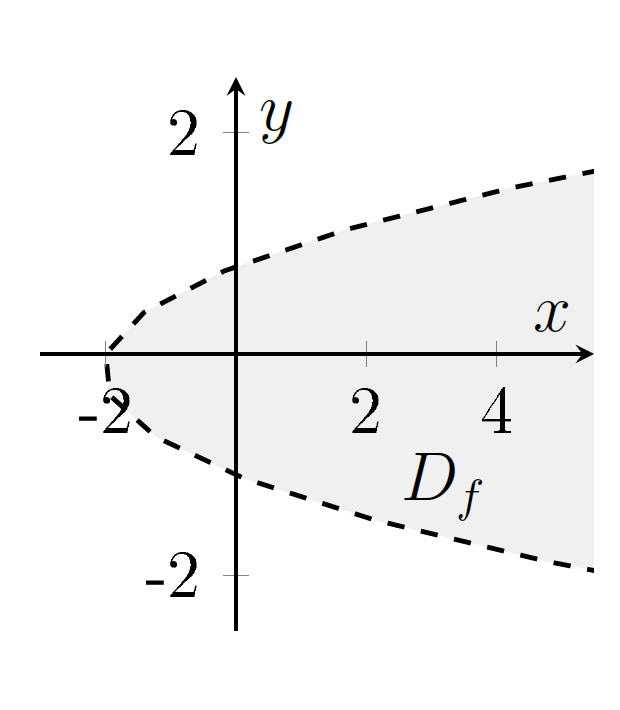
\includegraphics[scale=0.3]{pictures/BildA}
\item \text{} \\
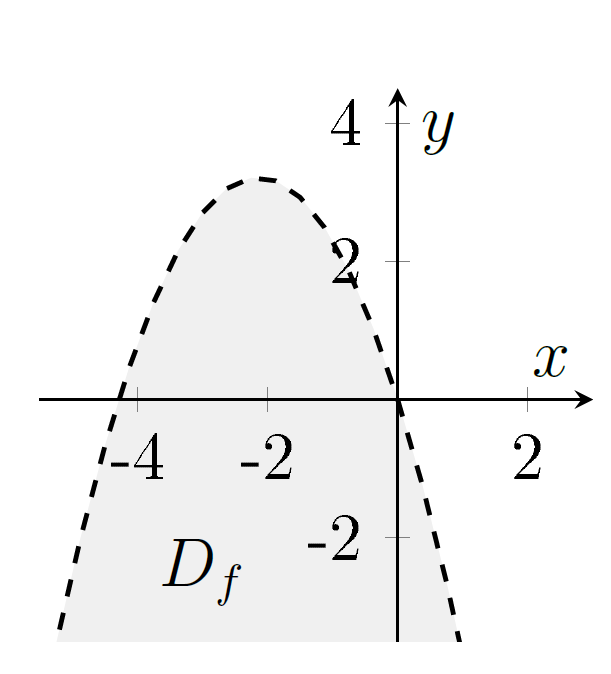
\includegraphics[scale=0.3]{pictures/BildB}
\item \text{} \\
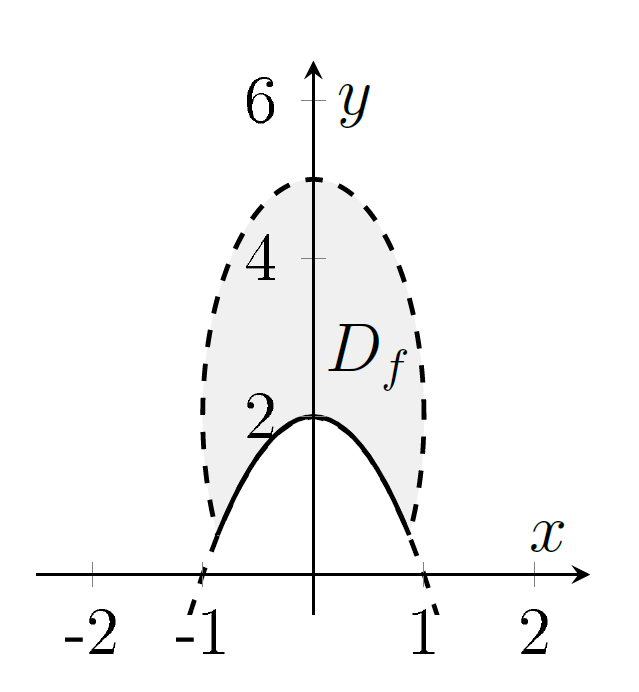
\includegraphics[scale=0.3]{pictures/BildC}
\item \text{} \\
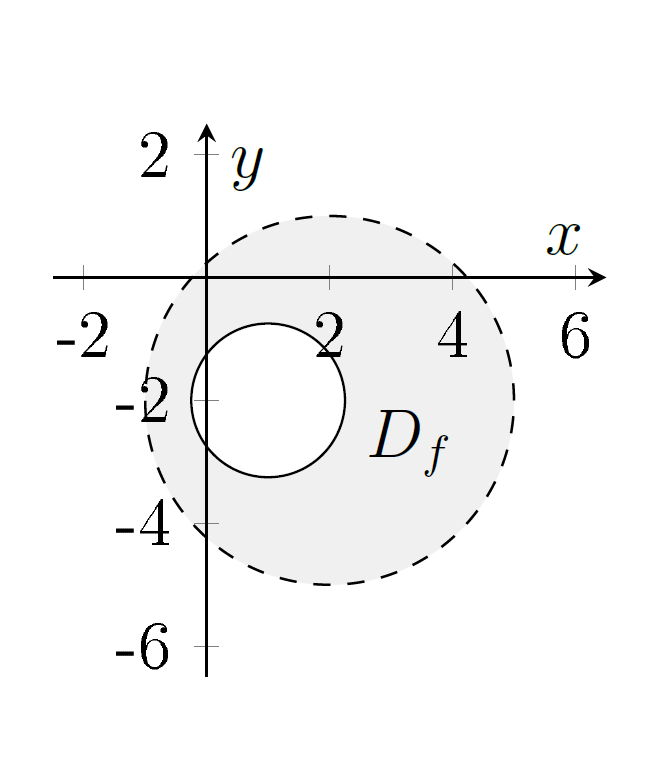
\includegraphics[scale=0.3]{pictures/BildD}
\end{enumerate}

\textbf{Lösung:}
\begin{mdframed}
\underline{\textbf{Vorgehensweise:}}
\renewcommand{\labelenumi}{\theenumi.}
\begin{enumerate}
\item Überlege, welche Bedingungen für den Definitionsbereich gelten müssen.
\item Alternative durch systematisches Ausschließen.
\end{enumerate}
\end{mdframed}

\underline{1. Überlege, welche Bedingungen für den Definitionsbereich gelten müssen}\\
Der Definitionsbereich des Logarithmus und der Wurzel liefern
\begin{align*}
-9x^2 -y^2 +4y +5 &> 0 
\ \text{und} \
4x^2 + 2y - 4 \geq 0
\end{align*}
als Bedingungen.
Die zweite Bedingung ist leichter handhabbar, weswegen wir mit dieser beginnen.
Mit
\begin{align*}
&\ \ \ \ 4x^2 + 2y -4 \geq 0\\ 
&\Leftrightarrow
2y \geq -4x^2 +4\\
&\Leftrightarrow
y \geq -2x^2 +2
\end{align*}
erhalten wir eine \glqq Funktionsvorschrift\grqq~für die zweite Bedingung.
Das bedeutet:
Durch $y = -2x^2 +2$ wird eine Parabel beschrieben.
Mit $y \geq -2x^2 +2 $ erhalten wir die $(x,y)$, welche auf oder über der Parabel liegen.
Die zweite Bedingung liefert uns durch
\begin{align*}
&\ \ \ -9x^2 -y^2 + 4 y +5 > 0\\
&\Leftrightarrow
5 > 9x^2 +y^2 -4y\\
&\Leftrightarrow
5 >9x^2 +y^2 -4y +4 -4\\
&\Leftrightarrow
9 > 9x^2 + (y-2)^2\\
&\Leftrightarrow
1 > x^2 + \frac{(y-2)^2}{9}\\
&\Leftrightarrow
\frac{x^2}{1^2} + \frac{(y-2)^2}{3^2} < 1
\end{align*}
eine Ellipse mit Zentrum $(0,2)$ und den Halbachsen $1$ in $x$-Richtung und $3$ in $y$-Richtung.
\\
\\

\underline{2. Alternative durch systematisches Ausschließen}\\
Das Wissen um die zweite Bedingung lässt uns nun direkt die 
Antworten (a), (b) und (d) auschließen.
Wir finden in allen Schaubildern Punkte, welche unterhalb des Graphen von $-2x^2 +2$ liegen.\\
\\

Somit ist Antwort (c) richtig.

\newpage

\subsection*{\frage{5}{3}}
Eine homogene Funktion vom Grad 2 habe die partielle Elastizität 
$\varepsilon_{f,x}$ gleich $5x+1$.
Es folgt, dass
\renewcommand{\labelenumi}{(\alph{enumi})}
\begin{enumerate}
\item $\varepsilon_{f,y}(x,y) = -5x +1$.
\item $\varepsilon_{f,y}(x,y) = 5x +1$.
\item $\varepsilon_{f,y}(x,y) = -5x +2$.
\item $\varepsilon_{f,y}(x,y) = 5x +1$.
\end{enumerate}
\ \\
\textbf{Lösung:}
\begin{mdframed}
\underline{\textbf{Vorgehensweise:}}
\renewcommand{\labelenumi}{\theenumi.}
\begin{enumerate}
\item Überlege, was laut Euler für homogene Funktionen vom Grad $k$ gilt.
\item Ermittle hiermit die richtige Antwort.
\end{enumerate}
\end{mdframed}

\underline{1. Überlege, was laut Euler für homogene Funktionen vom Grad $k$ gilt }\\
Wir wissen, dass der Zusammenhang
\begin{align*}
\varepsilon_{f,x}(x,y) + \varepsilon_{f,y}(x,y) = k
\end{align*}
für homogene Funktionen vom Grad $k$ laut Euler gilt.
\\ 
\\
\underline{2. Ermittle hiermit die richtige Antwort}\\
Durch Umformen und Einsetzen erhalten wir: 
\begin{align*}
\varepsilon_{f,y}(x,y) &= k - \varepsilon_{f,x}(x,y)\\
&= 2 - (5x +1)\\ &= 2 - 5x -1\\  &= -5x +1
\end{align*}

Somit ist Antwort (a) richtig.

\newpage 

\subsection*{\frage{6}{3}}
Gegeben sei die Funktion $f$ definiert durch
\begin{align*}
f(x,y) = \sqrt[5]{x^{3.4}y^{0.6}}+ \sqrt{x^{0.8}y^{0.8}} 
+ \sqrt[3]{x^{1.6}y^{0.7}}
\end{align*}
wobei $x >0$ und $y> 0$.
\renewcommand{\labelenumi}{(\alph{enumi})}
\begin{enumerate}
\item $f$ ist homogen vom Grad $0.6$.
\item $f$ ist homogen vom Grad $0.7$.
\item $f$ ist homogen vom Grad $0.8$.
\item $f$ ist nicht homogen.
	
\end{enumerate}
\ \\
\textbf{Lösung:}
\begin{mdframed}
\underline{\textbf{Vorgehensweise:}}
\renewcommand{\labelenumi}{\theenumi.}
\begin{enumerate}
\item Ermittle die allgemeine Homogenitätsbedingung.
\item Beweise, ob die Funktion homogen oder nicht homogen ist.
\end{enumerate}
\end{mdframed}

\underline{1. Ermittle die allgemeine Homogenitätsbedingung} \\
Eine Funktion $f \ : \ D_f  \to \mathbb{R}$ heißt homogen vom Grad $n$, falls
\begin{align*}
f(\lambda x, \lambda y) = \lambda^n \cdot f(x,y)
\end{align*}
für alle $x \in D_f$ und $\lambda > 0$ gilt.
\\
\\

\underline{2. Beweise, ob die Funktion homogen oder nicht homogen ist}\\
%Wir wählen ein beliebiges $\lambda >0 $. 
%Für $\lambda = 0 $ erhalten wir die Gleichung $0 = 0$, wodurch wir diesen Fall direkt auschließen können.
Durch Einsetzen erhalten wir:
\begin{align*}
f( \lambda x, \lambda y ) 
&= \sqrt[5]{(\lambda x)^{3.4} (\lambda y)^{0.6}}
  + \sqrt{(\lambda x)^{0.8} (\lambda y)^{0.8}}
  + \sqrt[3]{(\lambda x)^{1.6} (\lambda y)^{1.6}}\\
&=  \sqrt[5]{\lambda^{3.4} x^{3.4} \lambda^{0.6} y^{0.6}}
  + \sqrt{\lambda^{0.8} x^{0.8} \lambda^{0.8} y^{0.8}}
  + \sqrt[3]{\lambda^{1.6} x^{1.6} \lambda^{1.6} y^{1.6}}\\
&=  \sqrt[5]{\lambda^{4} x^{3.4} y^{0.6}}
  + \sqrt{\lambda^{1.6} x^{0.8}  y^{0.8}}
  + \sqrt[3]{\lambda^{3.2} x^{1.6} y^{1.6}}\\
&=  \lambda^{0.8} \sqrt[5]{ x^{3.4} y^{0.6}}
  + \lambda^{0.8} \sqrt{ x^{0.8}  y^{0.8}}
  + \lambda^{\frac{3.2}{3}} \sqrt[3]{ x^{1.6} y^{1.6}}\\
&=  \lambda^{0.8} \left( \sqrt[5]{ x^{3.4} y^{0.6}}
  + \sqrt{ x^{0.8}  y^{0.8}}
  + \lambda^{\frac{3.2}{3} -0.8} \sqrt[3]{ x^{1.6} y^{1.6}} \right)
\end{align*}
$f$ ist damit nicht homogen.\\
\\
Somit ist Antwort (d) richtig.
 
\newpage

\subsection*{\frage{7}{3}}
Gegeben sei die Funktion $f$ definiert durch
\begin{align*}
f(x,y) = x^{3.1} \sqrt{y} + 6 y^{3.5} \sqrt{ 5 x^{0.2}}
		+ x^a y^{2a}
\end{align*}
wobei $x > 0 $, $ y >0 $ und $a \in \mathbb{R}$.\\
Für welchen Wert von $a$ ist $f$ homogen?
\renewcommand{\labelenumi}{(\alph{enumi})}
\begin{enumerate}
\item $a = 1$.
\item $a = 1.2$.
\item $a = 1.4$.
\item $f$ ist für kein $a \in \mathbb{R}$ homogen.
	
\end{enumerate}
\ \\
\textbf{Lösung:}
\begin{mdframed}
\underline{\textbf{Vorgehensweise:}}
\renewcommand{\labelenumi}{\theenumi.}
\begin{enumerate}
\item Ermittle die allgemeine Homogenitätsbedingung.
\item Rechne die Definition der Homogenität nach.
\end{enumerate}
\end{mdframed}

\underline{1. Ermittle die allgemeine Homogenitätsbedingung} \\
Eine Funktion $f \ : \ D_f  \to \mathbb{R}$ heißt homogen vom Grad $n$, falls
\begin{align*}
f(\lambda x, \lambda y) = \lambda^n \cdot f(x,y)
\end{align*}
für alle $x \in D_f$ und $\lambda > 0$ gilt.
\\
\\

\underline{2. Rechne die Definition der Homogenität nach}\\
Durch Einsetzen erhalten wir:
\begin{align*}
f(\lambda x , \lambda y) 
&= (\lambda x )^{3.1} \sqrt{\lambda y}
	+ 6 (\lambda y)^{3.5} \sqrt{5 (\lambda x)^{0.2}}
	+(\lambda x)^a (\lambda y)^{2a}\\
&= \lambda^{3.1} x^{3.1}  \lambda^{0.5} \sqrt{ y}
	+ 6 \lambda^{3.5} y^{3.5} \sqrt{5 \lambda^{0.2} x^{0.2}}
	+\lambda^a x^a \lambda^{2a} y^{2a}\\
&= \lambda^{3.6} x^{3.1}  \sqrt{ y}
	+ 6 \lambda^{3.5} y^{3.5} \lambda^{0.1} \sqrt{5  x^{0.2}}
	+\lambda^{3a} x^a  y^{2a}\\
&= \lambda^{3.6} x^{3.1}  \sqrt{ y}
	+ 6 \lambda^{3.6} y^{3.5}  \sqrt{5  x^{0.2}}
	+\lambda^{3a} x^a  y^{2a}\\
&= \lambda^{3.6} \left( x^{3.1}  \sqrt{ y}
	+ 6 y^{3.5}  \sqrt{5  x^{0.2}}
	+\lambda^{3a - 3.6} x^a  y^{2a} \right)\\		
\end{align*}
Daraus resultiert die Bedingung $3a - 3.6 = 0$ für die Homogenität.
Mit 
\begin{align*}
&\ \ \ \ \ 3 a - 3.6 = 0\\
&\Leftrightarrow
3a = 3.6\\
&\Leftrightarrow
a = 1.2
\end{align*}
erhalten wir noch das dazu passende $a$.\\
\\
Somit ist Antwort (b) richtig.

\newpage

\subsection*{\frage{8}{2}}
Die Funktion zweier reeller Variablen $f$ ist homogen vom Grad $3$ und die Funktion zweier reeller Variablen $g$ ist homogen vom Grad $2$.
Die Funktion $h$ ist definiert durch
$h(x,y) = f\left( (g(x,y))^2, (g(x,y))^2 \right)$.
Dann gilt
\renewcommand{\labelenumi}{(\alph{enumi})}
\begin{enumerate}
\item $\varepsilon_{h,x}(x,y) + \varepsilon_{h,y}(x,y) = 3$.
\item $\varepsilon_{h,x}(x,y) + \varepsilon_{h,y}(x,y) = 6$.
\item $\varepsilon_{h,x}(x,y) + \varepsilon_{h,y}(x,y) = 12$.
\item $\varepsilon_{h,x}(x,y) + \varepsilon_{h,y}(x,y) = 18$.
\end{enumerate}
\ \\
\textbf{Lösung:}
\begin{mdframed}
\underline{\textbf{Vorgehensweise:}}
\renewcommand{\labelenumi}{\theenumi.}
\begin{enumerate}
\item Ermittle die allgemeine Homogenitätsbedingung.
\item Wende die Voraussetzung der Homogenität auf $h$ an.
\end{enumerate}
\end{mdframed}

\underline{1. Ermittle die allgemeine Homogenitätsbedingung} \\
Eine Funktion $f \ : \ D_f  \to \mathbb{R}$ heißt homogen vom Grad $n$, falls
\begin{align*}
f(\lambda x, \lambda y) = \lambda^n \cdot f(x,y)
\end{align*}
für alle $x \in D_f$ und $\lambda > 0$ gilt.
\\
\\

\underline{2. Wende die Voraussetzung der Homogenität auf $h$ an }\\
Durch Einsetzen erhalten wir:
\begin{align*}
h( \lambda x , \lambda y ) 
&= f \left( (g(\lambda x , \lambda y ))^2 , (g(\lambda x , \lambda y ))^2 \right)\\
&= f \left( ( \lambda^2 g(x,y) )^2, ( \lambda^2 g(x,y) )^2 \right)\\
&= f \left(  \lambda^4 (g(x,y) )^2, \lambda^4 (g(x,y) )^2 \right)
\\
&= \left(\lambda^4\right)^3 f \left(   (g(x,y) )^2,  (g(x,y) )^2 \right)\\
&= \lambda^{12} f \left(   (g(x,y) )^2,  (g(x,y) )^2 \right)\\
&= \lambda^{12} h(x,y)
\end{align*}
Somit ist die Funktion homogen vom Grad $12$. 
Es folgt 
\begin{align*}
\varepsilon_{h,x}(x,y) + \varepsilon_{h,y}(x,y) = 12
\end{align*}
mit der Relation von Euler.\\
\\
Somit ist Antwort (c) richtig.
